\documentclass[a4paper,10pt]{article}
\usepackage[utf8]{inputenc}
\usepackage[T1]{fontenc}	
\usepackage[italian]{babel}

\usepackage{amsmath}
\usepackage{amsfonts}
\usepackage{amssymb}
\usepackage{graphicx}

\usepackage[left=2cm,right=2cm,top=2cm,bottom=2cm]{geometry}
\geometry{a4paper}

\usepackage{booktabs}
\usepackage{verbatim}
\usepackage{subfig}
\usepackage{hyperref}


\usepackage[cdot, thickqspace, squaren]{SIunits}
\usepackage{float}
% macro
\def\code#1{\texttt{#1}}

\title{Esperienza di Ottica 1}
\author{Gruppo BL \\ Candido Alessandro, Luzio Andrea, Mazziotti Fabrizio}

\begin{document}

\maketitle

\section{Scopo}
L'esperienza è divisa in due parti:
\begin{itemize}
	\item nella prima parte si vuole determinare la lunghezza d’onda di una riga spettrale emessa dal sodio (la riga gialla);
	\item nella seconda parte ci sono due obiettivi:
	\begin{itemize}
		\item il primo è di valutare la risoluzione dello strumento di misura, uno spettroscopio a reticolo, nella misura delle linee emesse da lampade spettrali;
		\item il secondo è quello di determinare la costante di Rydberg dalla misura della lunghezza d’onda delle righe di emissione dell’idrogeno.
	\end{itemize}
\end{itemize}



\section{Esperienza A: Misura della lunghezza d'onda della riga gialla del sodio}

\subsection{Strumentazione}

\begin{itemize}
	\item spettroscopio a prisma:
	\begin{itemize}
		\item due telescopi;
		\item prisma con supporto;
		\item struttura di base, con possibilità di ruotare il supporto del prisma e blocco per la posizione, e possibilità di ruotare il telescopio d'osservazione, con blocco e goniometro dotato di nonio per la misura della posizione del telescopio stesso.
	\end{itemize}
	\item lampada al cadmio;
	\item lampada al sodio;
	\item lente d'ingrandimento, per la lettura del nonio;
	\item torcia.
\end{itemize}

\begin{figure}[H]
	\centering
	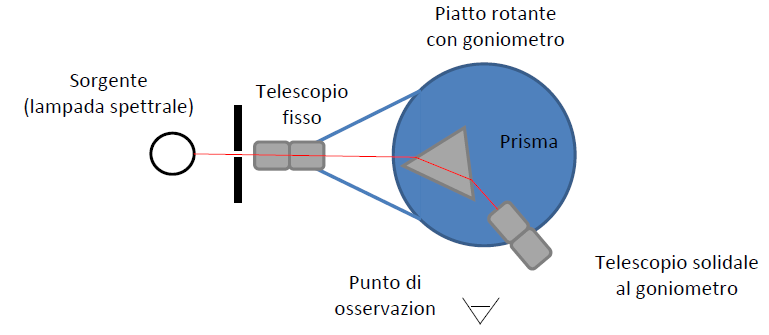
\includegraphics[width=0.7\textwidth]{../grafici/Schema1.png}
	\caption{Schema dell'apparato usato}
	\label{fig:schema1}
\end{figure}

\subsection{Calibrazione dello strumento con la lampada al cadmio}

Si è accesa la lampada al cadmio e dopo aver atteso qualche minuto, per far sì che andasse in temperatura, si sono eseguite le seguenti operazioni.

\paragraph{Determinazione dello "zero" del goniometro} Come prima cosa si è rimossa la torretta e si è posizionata approssimativamente la lampada in modo che la fessura raccogliesse più luce possibile. 

Si è dunque allineato il telescopio di osservazione e si è migliorato il posizionamento della lampada, decidendo assieme l'apertura della slitta d'ingresso. Per fare ciò si è riposizionato anche il prisma per verificare l'effetto dell'apertura della slitta sulla visualizzazione delle righe spettrali; un'apertura troppo ristretta non consentiva il passaggio di abbastanza luce, viceversa se troppo larga si aveva ambiguità sulla posizione della riga e, decisamente più importante, la luce delle righe più intense diventa troppa, al punto da peggiorare la visualizzazione di quelle meno intense.

Si è infine acquisito l'angolo ($\alpha_0$) a cui veniva osservata la luce non deflessa, a partire dall'uscita del telescopio fisso. Come indicato la misura è stata effettuata da tutti i componenti del gruppo, ottenendo così 3 misure, al fine di valutare l'errore sistematico associato al metodo di misura.
Si è trovato: $\alpha_0 = 10\degree~53.7'\pm 1.5'$

\begin{table}[H]
	\centering
	\begin{tabular}{c|c|c}
		$10\degree~55'$  & $10\degree~52'$ & $10\degree~54'$\\
	\end{tabular}
\caption{Dati raccolti sulla misura di $\alpha_0$}
\end{table}

Si è inoltre stimato indipendentemente che, data la larghezza dell'oculare, il singolo osservatore poteva compiere un errore massimo di parallasse pari a circa $2'-3'$ complessivi (ampiezza dell'intervallo), quindi circa $\pm 1'-1.5'$, si è in seguito supposto che fosse già incluso nelle fluttuazioni considerate con la misura da parte di più osservatori.

\paragraph{Determinazione della condizione di minima deviazione} Si è osservato lo spostamento delle righe spettrali del cadmio in funzione della posizione del prisma, e si è individuata la posizione corrispondente alla condizione di minimo spostamento relativa alla riga verde, la più vicina alla riga gialla attesa del sodio.

Si è notato che la posizione della riga verde era stazionaria, entro la sensibilità consentita dall'apparato, per un certo intervallo di posizioni del prisma, si è perciò sfruttata questa indeterminazione (più correttamente: si è cercato di ridurla) imponendo approssimativamente la condizione di minimo spostamento anche per la riga rossa.
L'inesattezza in quest'ultima operazione è introdotta dal fatto che fosse difficile per l'osservatore assicurare che la condizione, che veniva verificata dinamicamente ruotando il prisma, fosse rispettata da entrambe le righe; si è dunque privilegiato la riga verde, in quanto era stata individuata in principio come la più vicina alla zona d'interesse.

Il prisma è stato dunque bloccato nella posizione individuata, e non è stato più mosso nel seguito dell'esperienza A.

\paragraph{Calibrazione della scala spettrale} 

Si sono misurate le posizioni delle righe del cadmio nel modo descritto per l'individuazione dello zero. I valori di tutte le misure sono riportati in \tablename{~\ref{tab:cadmio}}.

\begin{table}[H]
	\centering
	\begin{tabular}{c|c|c|c}
	blu & azzurro & verde & rosso \\
	\hline
	$60\degree~39'$ & $60\degree~29'$ & $60\degree~0'$ & $58\degree~43'$\\
	$60\degree~40'$ & $60\degree~26'$ & $60\degree~0'$ & $58\degree~41'$\\
	$60\degree~41'$ & $60\degree~28'$ & $60\degree~0'$ & $58\degree~44'$\\
	\end{tabular}
	\caption{Misura delle righe del cadmio}
	\label{tab:cadmio}
\end{table}

Si è quindi eseguito un fit affine per la calibrazione della scala spettrale, si riporta il grafico in \figurename{~\ref{fig:cadmio}.

\begin{figure}[H]
	\centering
	\includegraphics[width=0.7\textwidth]{../grafici/calcadmio.pdf}
	\caption{Dati sperimentali e fit affine delle righe spettrali del cadmio}
	\label{fig:cadmio}
\end{figure}

I risultati ottenuti dal fit per coefficiente angolare ($m$) ed intercetta ($q$) sono riportati di seguito in \tablename{~\ref{tab:calcadmio}.
	

\begin{table}[H]
	\centering
	\begin{tabular}{|c|c|c|c|}
		\cline{0-1}		
		$m$ & $\unit{0.373 \pm 0.009}{eV/~\degree}$ \\
		\cline{0-1}
		$q$ & $\unit{-15.9 \pm 0.4}{eV}$ \\
		\hline
		$\chi^2$ & 4.59& ndof & 2\\
		\hline
	\end{tabular}
	\caption{Parametri ottenuti dal fit}
	\label{tab:calcadmio}
\end{table}

\subparagraph{Riga viola} Si è inoltre misurata un ulteriore riga nella regione viola dello spettro, l'intensità di questa riga era però molto debole, la misura è stata quindi notevolmente meno precisa.
Si riportano i dati raccolti in \tablename{~\ref{tab:viola}.
	
\begin{table}[H]
	\centering
	\begin{tabular}{c|c|c}
		$61\degree~15'$  & $61\degree~16'$ & $61\degree~11'$\\
	\end{tabular}
	\caption{Dati raccolti sulla riga viola}
	\label{tab:viola}
\end{table}
	
Non si è incluso questo valore nel fit perché non era a disposizione un valore corrispondente della lunghezza d'onda con cui confrontarlo.

\subsection{Misura della lunghezza d’onda della riga osservata del sodio}

\paragraph{Riga di emissione gialla}
Dopo aver posizionato la lampada al sodio seguendo gli stessi accorgimenti sopra descritti per la fenditura e la distanza da essa, si è misurata la sua riga di emissione nella regione gialla dello spettro, con la stessa modalità adottata per le righe del cadmio.
Si riportano le misure in \tablename{~\ref{tab:gialloNa}.

\begin{table}[H]
	\centering
	\begin{tabular}{c|c|c}
		$61\degree~15'$  & $61\degree~16'$ & $61\degree~11'$\\
	\end{tabular}
	\caption{Dati raccolti sulla riga viola}
	\label{tab:gialloNa}
\end{table}

Dalla calibrazione effettuata con il cadmio si ottiene che la lunghezza d'onda corrispondente alla riga è: $\lambda_{yellow, Na} = \unit{594 \pm 6}{\nano\meter}$, cioè ha un'energia pari a $E_{yellow, Na} = \unit{2.086\pm0.020}{e\volt}$.

\paragraph{Altre righe}

Si sono misurate anche altre righe emessa dalla lampada al sodio, si riportano in \tablename{~\ref{tab:moreNa} i vari valori e le relative lunghezze d'onda associate.

\begin{table}[H]
	\centering
	\begin{tabular}{c|c|c|c|c|c}
		colore &	&	&	& misura & lunghezza d'onda [nm]\\
		\hline
		rosso &	$58\degree~55'$ & $58\degree~53'$ & $58\degree~56'$ & $58\degree~54'~40'' \pm 1'~30''$ & $618 \pm 5$\\
		verde & $59\degree~18'$ & $59\degree~20'$ & $59\degree~16'$ & $59\degree~18' \pm 2'$  & $576 \pm 5$\\
		verde scuro & $59\degree~55'$ & $59\degree~55'$ & $59\degree~55'$ & $59\degree~55' \pm 1'$ & $520 \pm 9$\\
		azzurro & $60\degree~8'$ & $60\degree~10'$ & $60\degree~6'$ & $60\degree~8' \pm 2'$& $503 \pm 4$\\
		viola & $60\degree~39'$ & $60\degree~39'$ & $60\degree~39'$ & $60\degree~39' \pm 1'$ & $467 \pm 7$\\	
	\end{tabular}
	\caption{Misura delle ulteriori righe del sodio}
	\label{tab:moreNa}
\end{table}

L'intensità delle altre righe era per tutte minore rispetto a quella della riga gialla, ma alcune erano comunque ben visibili, mentre, anche in questo caso, la riga nella regione viola dello spettro lo era poco.

Si è provato a migliorare la visualizzazione della riga viola muovendo la slitta d'ingresso, ottenendo però modesti risultati.

\subparagraph{Osservazione} Confrontando gli spettri noti non tutte le righe sono ascrivibili alle transizioni elettroniche del sodio atomico, è probabile che le righe in più siano dovute ad impurezze nel campione emittente. Maggiori informazioni a riguardo si possono ottenere nella sezione "Curiosità: linee non note" della seconda parte dell'esperimento in quanto simili linee sono state trovate anche nello spettro della lampada a idrogeno.


\section{Esperienza B: Stima della costante di Rydberg}
\subsection{Scopo}
Lo scopo di questa esperienza è misurare la costante di Rydberg attraverso la misura delle lunghezze d'onda delle linee spettrali della serie di Balmer dell'idrogeno. Ciò viene fatto attraverso uno spettroscopio a reticolo di diffrazione (in riflessione) precedentemente calibrato con una lampada spettroscopica al mercurio. Viene poi stimata la risoluzione dello strumento attraverso l'osservazione del doppietto D del sodio.
\subsection{Strumentazione}

\begin{itemize}
	\item spettroscopio a reticolo di diffrazione:
	\begin{itemize}
		\item due telescopi;
		\item prisma con supporto;
		\item struttura di base, con possibilità di ruotare il supporto del prisma e blocco per la posizione, e possibilità di ruotare il telescopio d'osservazione, con blocco e goniometro dotato di nonio per la misura della posizione del telescopio stesso.
	\end{itemize}
	\item lampada al mercurio;
	\item lampada al idrogeno;
	\item lampada al sodio;
	\item lente d'ingrandimento, per la lettura del nonio;
	\item torcia.
\end{itemize}

\begin{figure}[H]
	\centering
	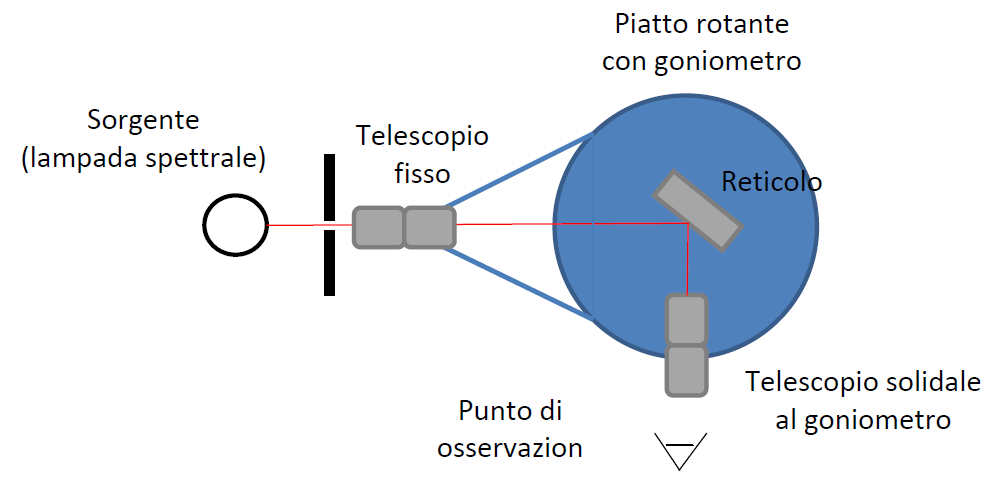
\includegraphics[width=0.7\textwidth]{../grafici/Schema2.png}
	\caption{Schema dell'apparato usato}
	\label{fig:schema2}
\end{figure}

\subsection{Regolazione della geometria dei telescopi}
Lo schema dell'apparato è rappresentato in figura \figurename{~\ref{fig:schema2}}.

In primo luogo si è posizionata la lampada al mercurio vicino al telescopio fisso e si è ruotato il telescopio di osservazione fino ad osservare l'ordine zero di diffrazione. Si è fissato questo telescopio e si è regolato lo spessore della fenditura, la distanza della lampada da essa e la messa a fuoco del telescopio per visualizzare la riga con la maggior intensità possibile e con uno spessore né troppo piccolo da non permettere la visualizzazione della riga, né troppo grande per evitare che le righe più luminose peggiorassero la visibilità di quelle meno intense. La distanza della lampada dalla fenditura non deve essere né troppo grande ($\sim 1 cm$) perché ne risentirebbe la luminosità delle riga, né troppo piccola perché si vedrebbero aloni intorno ad essa.
Si sono poi osservate le righe del primo ordine di diffrazione (quelle più intense,cioè, in ordine per angolo di incidenza decrescente: viola, verde, rosso e un doppietto giallo) e si è verificato che, con gli stessi accorgimenti fatti per la riga dell'ordine zero, esse siano ben messe a fuoco.

\subsection{Calibrazione dello strumento e misura del passo reticolare}
Con la stessa procedura effettuata nella parte A si è effettuata la calibrazione del nonio ottenendo $\alpha_0 = 348\degree 42' \pm  2' $\footnote{La trattazione dei vari dati acquisiti in questa parte dell'esperienza e dei relativi errori,ove non specificato, è stata trattata allo stesso modo di come descritto nella parte A.}. Presa questa misura, tutte le letture successive fatte sul nonio e riportate qui saranno riferite a questo valore.


\paragraph{Misura del passo reticolare}
Il passo reticolare è stato misurato conoscendo la lunghezza d'onda della riga verde del sodio. Sono stati misurati, relativamente all'angolo di calibrazione $\alpha_0$, l'angolo della riflessione speculare e del primo massimo di interferenza della riga verde del mercurio: $\theta_{i,ord0} = 8\degree 55.7' \pm 0.5'$, $\theta_{i,ord1} = 69\degree 29.0'\pm 1'$. Nota la lunghezza d'onda della suddetta linea ($546.074 \pm 0.001 nm$) per stimare il passo reticolare $d$ si sono utilizzate le equazioni
\begin{align*}
&d(sin \theta_{i,ord0} - sin \theta_d) = m\lambda\\
&\theta_{i,ord0} = (\pi - \alpha_0)/2\\
&\theta_d = \pi - \theta_{i,ord1} - \alpha_1
\end{align*}

Una rappresentazione schematica per trovare le ultime due equazioni precedenti è mostrata in \figurename{~\ref{fig:angoli}}. La prima equazione è quella nota che lega il passo reticolare all'ordine di diffrazione m e alla lunghezza d'onda $\lambda$.


\begin{figure}[H]
	\centering
	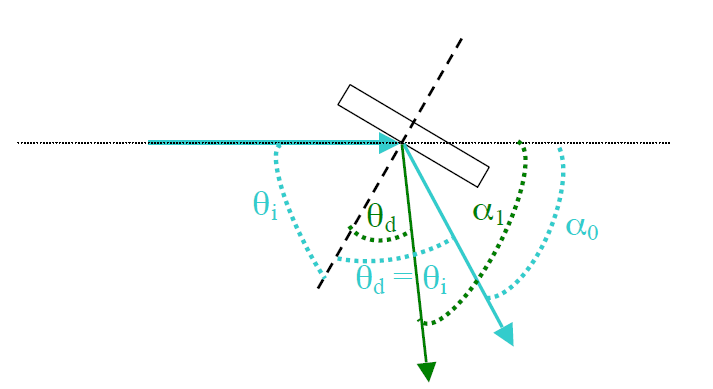
\includegraphics[width=0.7\textwidth]{../grafici/Angoli.png}
	\caption{Rappresentazione schematica degli angoli utlizzati per trovare il passo reticolare $d$.}
	\label{fig:angoli}
\end{figure}

Gli errori sono stati propagati tenendo conto delle covarianze e i dati presi sono stati considerati con errori statistici\footnote{Si è ritenuto possibile considerare gli errori come statistici in quanto frutto della media di dati presi da persone diverse. Fra le prese dati dei vari elementi del gruppo si ha avuto cura di riportare il telescopio di osservazione in una zona neutra, in modo di evitare eventuali influenze da parte di membri del gruppo su altri.} e scorrelati. 
Il risultato ottenuto è dunque $d=835.57 \pm 0.25 nm$, ovvero $1196.8 \pm 0.4$ linee per mm. Il risultato sembra compatibile con quanto atteso ($\sim 1200$ linee per mm).

\subsection{Righe di emissione dell'idrogeno}

Per misurare la lunghezza d'onda delle linee dell'idrogeno si è deciso di diminuire l'angolo di incidenza del fascio entrante sul reticolo. Questo
dovrebbe aumentare la potenza delle righe osservate. Si è misurato un angolo di deviazione in riflessione di $46\degree 3' \pm 2'$. Riferite a tale angolo sono state misurate le posizioni angolari delle varie righe, che sono riportate in \tablename{~\ref{tab:HH}.

\begin{table}[H]
	\centering
	\begin{tabular}{c|c|c|c|c|c|c}
colore & $\alpha_1$ &	$\theta_d$ & ordine di diffrazione & $\lambda$[nm] & $\lambda_{attesa}$[nm]& $n_2$  \\
		\hline
azzurro &  $ 93\degree 7.0' \pm 4.0 ' $  &  $ 19\degree 54.0' \pm 4.0 ' $  &  $ 1 $ & $ 484.5 \pm 1.0 $ & $ 486.0 $ & $ 4 $\\
rosso &  $ 105\degree 16.0' \pm 4.0 ' $  &  $ 7\degree 45.0' \pm 4.0 ' $  &  $ 1 $ & $ 656.3 \pm 1.0 $ & $ 656.1 $ & $ 3 $\\
azzurro &  $ 127\degree 13.0' \pm 4.0 ' $  &  $ -15\degree 48.0' \pm 4.0 ' $  &  $ 2 $ & $ 486.9 \pm 0.5 $ & $ 486.0 $ & $ 4 $\\
d-viola &  $ 119\degree 18.0' \pm 3.0 ' $  &  $ -7\degree 43.0' \pm 3.0 ' $  &  $ 2 $ & $ 430.2 \pm 0.4 $ & $ 433.9 $ & $ 5 $\\
	\end{tabular}
	\caption{Misura delle righe spettrali dell'idrogeno. I nomi degli angoli sono gli stessi della \figurename{~\ref{fig:angoli} }.La d nel nome significa che in realtà la linea è un doppietto, di cui un componente è talmente fioco da non poter essere misurato.}
	\label{tab:HH}
\end{table}

Si noti come il primo azzurro e il secondo dovrebbero essere la stessa linea spettrale viste al primo e al secondo massimo di interferenza. I valori sono compatibili tra loro entro 2 sigma.
I valori di $n_1$ e $n_2$ sono quelli che compaiono nell'equazione

\begin{equation}
 1/\lambda=Ry(1/n_1^2-1/n_2^2)
\end{equation} 
 
La serie Balmer corrisponde a $n_2=2$, mentre per $n_2=1$ si ha la serie Lyman, ecc.	

La stima dei numeri quantici coinvolti è stata fatta con la misura di riferimento della costante di Rydberg\footnote{ Questo valore è privo della correzione apportata dalla massa finita del nucleo dell'ordine del 1 per mille.}: $Ry=1.097373156 * 10^{-2} nm^{-1}$. 


Si noti inoltre che sono state prese altre linee non compatibili con nessuna linea nota dell'idrogeno. I dati relativi a queste linee e le diverse ipotesi riguardo la loro origine sono discusse nella sezione "Curiosità: linee non note".


Dalle misure fatte si è proceduto con un fit della costante di Rydberg $Ry$. Si è fittata l'equazione (1) con i numeri quantici trovati in precedenza e riportati in \tablename{~\ref{tab:HH}, ottenendo i seguenti risultati:\\
$Ry= 0.01098 \pm 0.0007 nm^{-1}$ \\
$\chi^2=60.1$ (d.o.f.=3)

 

\begin{figure}[H]
	\centering
	\includegraphics[width=0.7\textwidth]{../grafici/Ryf.pdf}
	\caption{Fit dell'equazione $1/\lambda=Ry(1/n_1^2-1/n_2^2)$ per la determinazione di $Ry$}
	\label{fig:Idrogeno, serie Balmer}
\end{figure}

Si nota subito che il $\chi^2$ sia completamente fuori scala. Questo è anche ben visibile dal plot dei residui normalizzati \ref{fig:Idrogeno, Residui normalizzati}. Si ritiene che ciò sia dovuto alla difficoltà di misura della posizione delle righe rispetto alla croce del telescopio, in quanto esse non erano molto fioche. E' possibile dunque che gli errori siano stati sottostimati.

\begin{figure}[H]
	\centering
	\includegraphics[width=0.7\textwidth]{../grafici/Ryfr.pdf}
	\caption{Residui normalizzati del fit dell'equazione $1/\lambda=Ry(1/n_1^2-1/n_2^2)$ per la determinazione di $Ry$}
	\label{fig:Idrogeno, Residui normalizzati}
\end{figure}


Ciò nonostante il valore ottenuto della costante di Rydberg, da confrontare con il valore atteso di $0.010973 nm^{-1}$ (o meglio $0.010968 nm^{-1}$, correzione dovuta alla massa ridotta dell'idrogeno) è compatibile nell'errore sperimentale.
 

\subsection{Misura del doppietto del sodio}
A questo punto si è sostituita all lampada ad idrogeno la lampada al sodio. Ci si è focalizzati sul doppietto giallo (tra l'altro l'unico doppietto visibile che è realmente attribuibile al sodio). Nella tabella sotto \ref{tab:NaR} sono riportati gli angoli e le lunghezze ottenute.

\begin{table}[H]
	\centering
	\begin{tabular}{c|c|c|c}
		$\theta_i$ & $\lambda$[nm] & $\lambda_{attesa}$[nm]  \\
		\hline
  $ 12\degree 25.0' \pm 2.0 ' $ & $ 589.2 \pm 0.6 $ & $ 589.0 $ \\
  $ 12\degree 22.0' \pm 2.0 ' $ & $ 589.9 \pm 0.6 $ & $ 589.6 $ \\
\end{tabular}
	\caption{Doppietto del sodio. Nomi degli angoli seguono le convenzioni dei paragrafi precedenti}
	\label{tab:NaR}
\end{table}

La differenza fra le linee risulta essere dunque di $0.7\pm 0.7 nm$ (dove l'errore è stato propagato con la stessa procedura ottenuta in precedenza), da confrontare con il valore noto di $0.6 nm$. Questo farebbe pensare a una sovrastima dell'errore. Inoltre si può notare dalla tabella \ref{tab:NaR} che anche per il valore delle singole righe l'errore sembra essere sovrastimato: risultano entrambe spostate al più di $0.3 nm$, la metà dell'errore stimato.
Questo dovrebbe far credere che gli errori presenti in tabella \ref{tab:HH} (tutti dell'ordine del $nm$)debbano essere sbagliati di un fattore 5. Si noti però che una correzione di un fattore 5 negli errori porterebbe il valore del $\chi^2$ del fit della costante di Rydberg totalmente fuoriscala. D'altro canto bisogna osservare che le linee del sodio sono molto più intense di molte delle linee tabulate in \ref{tab:HH}, per alcune delle quali è stato difficile allineare la croce del centro del telescopio con la linea stessa. In particolare è stato molto difficile riconoscere l'allinearsi sulle linee del secondo ordine di diffrazione.


La differenza con la misura effettuata nella parte A è non solo quantitativa, ma addirittura qualitativa: con lo spettroscopio a prisma non si riesce ad apprezzare la presenza di due linee, cosa tra l'alto plausibile avendo una risoluzione di circa $6 nm$. Con il presente le due righe, distanti solo $0.6 nm$, sono chiaramente separate. Si stima dunque che lo spettroscopio a reticolo sia tra le 10 e le 100 volte più risolvente di quello a prisma.  




\label{Curiosità: linee non note}\subsection{Curiosità: linee non note}
Nella presa dati per l'idrogeno, oltre alle ben note linee della serie Balmer sono state viste altre linee meno note. \'E stato ipotizzato che tali linee siano originate:
\begin{itemize}
\item contaminazione di luce ambientale, per esempio le due lampade messe a riscaldare dietro il paravento
\item altri elementi presenti nella scarica della lampada, es. atomi di elettrodo, ossigeno o azoto dell'aria penetrati nella lampada.
\item linee dell'idrogeno molecolare.
\end{itemize}

In tabella \ref{tab:Cur} le linee ignote.


\begin{table}[H]
\centering
\begin{tabular}{c|c|c|c|c|c}
colore & $\theta_i$ & ordine & lunghezza d'onda [nm] & sodio[nm](esperimento 1) \\
\hline
d-verde&  $ 16\degree 43.0' \pm 3.0 ' $   &  $ 1 $ & $ 528.5 \pm 0.8 $  & $520 \pm 9$\\
rosso  &  $ 10\degree 32.0' \pm 2.0 ' $  &  $ 1 $ & $ 616.1 \pm 0.6 $ & $ 618 \pm 5 $\\
\end{tabular}
\caption{Misure delle righe ignote. La d nel nome significa che in realtà la linea è un doppietto, di cui un componente è talmente fioco da non poter essere misurato. Per semplicità sono state riportate le lunghezze d'onda delle righe corrispondenti in tabella \ref{tab:moreNa}, misurate con la lampada al sodio.}
\label{tab:Cur}
\end{table}

Si è scartata la prima ipotesi notando che gli spettri non appartengono ne al cadmio ne al mercurio.\footnote{Tutte le linee spettrali sono state confrontate con quelle tabulate dal sito \url{http://physics.nist.gov/PhysRefData/ASD/lines_form.html}}\\


La cosa più curiosa è che le stesse linee sono state osservate nella lampada al sodio usata per parte A dell'esperienza (linee presenti nella tabella \ref{tab:moreNa}s).

Dunque non essendo linee del sodio viene il sospetto che tali linee siano dovute a una qualche contaminazione presente in tutte e due le lampade. Si è dunque scartata la possibile presenza d'aria controllando lo spettro dell'azoto. Per quanto riguarda l'ossigeno, in effetti si è trovata una possibile corrispondenza con le righe osservate e riportate in \ref{tab:Cur}. Infatti per la riga rossa esistono tre righe di lunghezza d'onda simili ($\sim$ 615 nm, separazione di $\sim$ 0.1 nm) che sono in ottimo accordo con la riga misurata, mentre per quella d-verde si ha una buona corrispondenza con righe che hanno lunghezza d'onda di circa 532 nm.\footnote{In effetti ciò che si è osservato è un doppietto verde, di cui una delle due righe non era misurabile, e questo è in linea con quanto trovato sul sito di riferimento}. Le linee osservate dovrebbero essere dunque quelle presenti nei siti: \url . \\

Un'altra possibilità è che le linee appartengano agli atomi degli elettrodi o all'idrogeno molecolare. 

Il primo caso è però escluso in quanto il datasheet delle lampade sostiene che gli elettrodi siano in  tungsteno, e neanche il tungsteno sembra possedere quelle due linee spettrali.

Per il secondo caso non è stato possibile reperire dati.

\end{document}